%%%%%%%%%%%%%%%%%%%%%%%%%%%%%%%%%%%%%%%%%%%%%%%%%%%%%%%%%%%%%%%%%%%%%%%%%%%%%%%%
%%                                                                            %%
%%                                                                            %%
%% An example for writting your thesis using LaTeX                            %%
%% Original version and development work by Luis Costa, changes to the text   %% 
%% in the Finnish template by Perttu Puska.                                   %%
%% Support for Swedish added 15092014                                         %%
%% PDF/A-b support added on 15092017                                          %%
%% PDF/A-2 support added on 24042018                                          %%
%%                                                                            %%
%% This example consists of the files                                         %%
%%         thesistemplate.tex (version 3.20) (for text in English)            %%
%%         opinnaytepohja.tex (version 3.20) (for text in Finnish)            %%
%%         kandidatarbetsbotten.tex (version 1.00) (for text in Swedish)      %%
%%         aaltothesis.cls (versio 3.20)                                      %%
%%         kuva1.eps (graphics file)                                          %%
%%         kuva2.eps (graphics file)                                          %%
%%         kuva1.jpg (graphics file)                                          %%
%%         kuva2.jpg (graphics file)                                          %%
%%         kuva1.png (graphics file)                                          %%
%%         kuva2.png (graphics file)                                          %%
%%         kuva1.pdf (graphics file)                                          %%
%%         kuva2.pdf (graphics file)                                          %%
%%                                                                            %%
%%                                                                            %%
%% Typeset in Linux either with                                               %%
%% pdflatex: (recommended method)                                             %%
%%             $ pdflatex thesistemplate                                      %%
%%             $ pdflatex thesistemplate                                      %%
%%                                                                            %%
%%   The result is the file thesistemplate.pdf that is PDF/A compliant, if    %%
%%   you have chosen the proper \documenclass options (see comments below)    %%
%%   and your included graphics files have no problems.
%%                                                                            %%
%% Or                                                                         %%
%% latex: (this method is not recommended)                                    %%
%%             $ latex thesistemplate                                         %%
%%             $ latex thesistemplate                                         %%
%%                                                                            %%
%%   The result is the file thesistemplate.dvi, which is converted to ps      %%
%%   format as follows:                                                       %%
%%                                                                            %%
%%             $ dvips thesistemplate -o                                      %%
%%                                                                            %%
%%   and then to pdf as follows:                                              %%
%%                                                                            %%
%%             $ ps2pdf thesistemplate.ps                                     %%
%%                                                                            %%
%%   This pdf file is not PDF/A compliant. You must must make it so using,    %%
%%   e.g., Acrobat Pro or PDF-XChange.                                        %%
%%                                                                            %%
%%                                                                            %%
%% Explanatory comments in this example begin with the characters %%, and     %%
%% changes that the user can make with the character %                        %%
%%                                                                            %%
%%%%%%%%%%%%%%%%%%%%%%%%%%%%%%%%%%%%%%%%%%%%%%%%%%%%%%%%%%%%%%%%%%%%%%%%%%%%%%%%
%%%%%%%%%%%%%%%%%%%%%%%%%%%%%%%%%%%%%%%%%%%%%%%%%%%%%%%%%%%%%%%%%%%%%%%%%%%%%%%%
%%
%% WHAT is PDF/A
%%
%% PDF/A is the ISO-standardized version of the pdf. The standard's goal is to
%% ensure that he file is reproducable even after a long time. PDF/A differs
%% from pdf in that it allows only those pdf features that support long-term
%% archiving of a file. For example, PDF/A requires that all used fonts are
%% embedded in the file, whereas a normal pdf can contain only a link to the
%% fonts in the system of the reader of the file. PDF/A also requires, among
%% other things, data on colour definition and the encryption used.
%% Currently three PDF/A standards exist:
%% PDF/A-1: based on PDF 1.4, standard ISO19005-1, published in 2005.
%%          Includes all the requirements essential for long-term archiving.
%% PDF/A-2: based on PDF 1.7, standard ISO19005-2, published in 2011.
%%          In addition to the above, it supports embedding of OpenType fonts,
%%          transparency in the colour definition and digital signatures.
%% PDF/A-3: based on PDF 1.7, standard ISO19005-3, published in 2012.
%%          Differs from the above only in that it allows embedding of files in
%%          any format (e.g., xml, csv, cad, spreadsheet or wordprocessing
%%          formats) into the pdf file.
%% PDF/A-1 files are not necessarily PDF/A-2 -compatible and PDF/A-2 are not
%% necessarily PDF/A-1 -compatible.
%% All of the above PDF/A standards have two levels:
%% b: (basic) requires that the visual appearance of the document is reliably
%%    reproduceable.
%% a (accessible) in addition to the b-level requirements, specifies how
%%   accessible the pdf file is to assistive software, say, for the physically
%%   impaired.
%% For more details on PDF/A, see, e.g., https://en.wikipedia.org/wiki/PDF/A
%%
%%
%% WHICH PDF/A standard should my thesis conform to?
%%
%% Primarily to the PDF/A-1b standard. All the figures and graphs typically
%% use in thesis work do not require transparency features, a basic '2-D'
%% visualisation suffices. The font to be used are specified in this template
%% and they should not be changed. However, if you have figures where
%% transparency characteristics matter, use the PDF/A-2b standard. Do not use
%% the PDF/A-3b standard for your thesis.
%%
%%
%% WHAT graphics format can I use to produce my PDF/A compliant file?
%%
%% When using pdflatex to compile your work, use jpg, png or pdf files. You may
%% have PDF/A compliance problems with figures in pdf format. Do not use PDF/A
%% compliant graphics files.
%% If you decide to use latex to compile your work, the only acceptable file
%% format for your figure is eps. DO NOT use the ps format for your figures.

%% USE one of these:
%% * the first when using pdflatex, which directly typesets your document in the
%%   chosen pdf/a format and you want to publish your thesis online,

%% * the second when you want to print your thesis to bind it, or
%% * the third when producing a ps file and a pdf/a from it.
%%
\documentclass[english, 12pt, a4paper, sci, utf8, a-1b, online]{aaltothesis}
%\documentclass[english, 12pt, a4paper, elec, utf8, a-1b]{aaltothesis}
%\documentclass[english, 12pt, a4paper, elec, dvips, online]{aaltothesis}

%% Use the following options in the \documentclass macro above:
%% your school: arts, biz, chem, elec, eng, sci
%% the character encoding scheme used by your editor: utf8, latin1
%% thesis language: english, finnish, swedish
%% make an archiveable PDF/A-1b or PDF/A-2b compliant file: a-1b, a-2b
%%                    (with pdflatex, a normal pdf containing metadata is
%%                     produced without the a-*b option)
%% typeset in symmetric layout and blue hypertext for online publication: online
%%            (no option is the default, resulting in a wide margin on the
%%             binding side of the page and black hypertext)
%% two-sided printing: twoside (default is one-sided printing)
%%

\usepackage{graphicx}

%% Math fonts, symbols, and formatting; these are usually needed
\usepackage{amsfonts,amssymb,amsbsy,amsmath}

%% Change the school field to specify your school if the automatically set name
%% is wrong
% \university{aalto-yliopisto}
% \school{Sähkötekniikan korkeakoulu}

%% Edit to conform to your degree programme
%%
\degreeprogram{Master's Programme in ICT Innovation}
%%

%% Your major
%%
\major{Data Science}
%%

%% Major subject code
%%
\code{SCI3115}
%%
 
%% Choose one of the three below
%%
%\univdegree{BSc}
\univdegree{MSc}
%\univdegree{Lic}
%%

%% Your name (self explanatory...)
%%
\thesisauthor{Cristian Manuel Abrante Dorta}
%%

%% Your thesis title comes here and possibly again together with the Finnish or
%% Swedish abstract. Do not hyphenate the title, and avoid writing too long a
%% title. Should LaTeX typeset a long title unsatisfactorily, you mght have to
%% force a linebreak using the \\ control characters.
%% In this case...
%% Remember, the title should not be hyphenated!
%% A possible "and" in the title should not be the last word in the line, it
%% begins the next line.
%% Specify the title again without the linebreak characters in the optional
%% argument in box brackets. This is done because the title is part of the 
%% metadata in the pdf/a file, and the metadata cannot contain linebreaks.
%%
\thesistitle{Cristian Abrante's amazing thesis}
%\thesistitle[Title of the thesis]{Title of\\ the thesis}
%%

%%
\place{Otaniemi}
%%

%% The date for the bachelor's thesis is the day it is presented
%%
\date{31.12.2020}
%%

%% Thesis supervisor
%% Note the "\" character in the title after the period and before the space
%% and the following character string.
%% This is because the period is not the end of a sentence after which a
%% slightly longer space follows, but what is desired is a regular interword
%% space.
%%
\supervisor{Prof.\ Hong-Linh Truong}
%%

%% Advisor(s)---two at the most---of the thesis. Check with your supervisor how
%% many official advisors you can have.
%%
\advisor{Teemu Sidoroff}
%%

%% Aaltologo: syntax:
%% \uselogo{aaltoRed|aaltoBlue|aaltoYellow|aaltoGray|aaltoGrayScale}{?|!|''}
%% The logo language is set to be the same as the thesis language.
%%
\uselogo{aaltoRed}{''}
%%

%% The English abstract:
%% All the details (name, title, etc.) on the abstract page appear as specified
%% above.
%% Thesis keywords:
%% Note! The keywords are separated using the \spc macro
%%
\keywords{For keywords choose\spc concepts that are\spc central to your\spc thesis}
%%

%% The abstract text. This text is included in the metadata of the pdf file as well
%% as the abstract page.
%%
\thesisabstract{
Your abstract in English. Keep the abstract short. The abstract explains your 
research topic, the methods you have used, and the results you obtained. In the 
PDF/A format of this thesis, in addition to the abstract page, the abstract text is 
written into the pdf file's metadata. Write here the text that goes into the 
metadata. The metadata cannot contain special characters, linebreak or paragraph 
break characters, so these must not be used here. If your abstract does not contain 
special characters and it does not require paragraphs, you may take advantage of 
the abstracttext macro (see the comment below). Otherwise, the metadata abstract 
text must be identical to the text on the abstract page.
}

%% Copyright text. Copyright of a work is with the creator/author of the work
%% regardless of whether the copyright mark is explicitly in the work or not.
%% You may, if you wish, publish your work under a Creative Commons license (see
%% creaticecommons.org), in which case the license text must be visible in the
%% work. Write here the copyright text you want. It is written into the metadata
%% of the pdf file as well.
%% Syntax:
%% \copyrigthtext{metadata text}{text visible on the page}
%% 
%% In the macro below, the text written in the metadata must have a \noexpand
%% macro before the \copyright special character, and macros (\copyright and
%% \year here) must be separated by the \ character (space chacter) from the
%% text that follows. The macros in the argument of the \copyrighttext macro
%% automatically insert the year and the author's name. (Note! \ThesisAuthor is
%% an internal macro of the aaltothesis.cls class file).
%% Of course, the same text could have simply been written as
%% \copyrighttext{Copyright \noexpand\copyright\ 2018 Eddie Engineer}
%% {Copyright \copyright{} 2018 Eddie Engineer}
%%
\copyrighttext{Copyright \noexpand\copyright\ \number\year\ \ThesisAuthor}
{Copyright \copyright{} \number\year{} \ThesisAuthor}

%% You can prevent LaTeX from writing into the xmpdata file (it contains all the 
%% metadata to be written into the pdf file) by setting the writexmpdata switch
%% to 'false'. This allows you to write the metadata in the correct format
%% directly into the file thesistemplate.xmpdata.
%\setboolean{writexmpdatafile}{false}

%% All that is printed on paper starts here
%%
\begin{document}

%% Create the coverpage
%%
\makecoverpage

%% Typeset the copyright text.
%% If you wish, you may leave out the copyright text from the human-readable
%% page of the pdf file. This may seem like a attractive idea for the printed
%% document especially if "Copyright (c) yyyy Eddie Engineer" is the only text
%% on the page. However, the recommendation is to print this copyright text.
%%
\makecopyrightpage

%% Note that when writting your thesis in English, place the English abstract
%% first followed by the possible Finnish or Swedish abstract.

%% Abstract text
%% All the details (name, title, etc.) on the abstract page appear as specified
%% above.
%%
\begin{abstractpage}[english]
  Your abstract in English. Keep the abstract short. The abstract explains your
  research topic, the methods you have used, and the results you obtained.  
  
  The abstract text of this thesis is written on the readable abstract page as
  well as into the pdf file's metadata via the $\backslash$thesisabstract macro
  (see above). Write here the text that goes onto the readable abstract page.
  You can have special characters, linebreaks, and paragraphs here. Otherwise,
  this abstract text must be identical to the metadata abstract text.
  
  If your abstract does not contain special characters and it does not require
  paragraphs, you may take advantage of the abstracttext macro (see the comment
  below).
\end{abstractpage}

%% The text in the \thesisabstract macro is stored in the macro \abstractext, so
%% you can use the text metadata abstract directly as follows:
%%
%\begin{abstractpage}[english]
%	\abstracttext{}
%\end{abstractpage}

%% Force a new page so that the possible Finnish or Swedish abstract does not
%% begin on the same page
%%
\newpage

%% Preface
%%
%% This section is optional. Remove it if you do not want a preface.
\mysection{Preface}

I want to thank Professor Pirjo Professori and my instructor Dr Alan Advisor for 
their good and poor guidance.\\

\vspace{5cm}
Otaniemi, 31.12.2020

\vspace{5mm}
{\hfill Cristian M.\ Abrante Dorta \hspace{1cm}}

%% Force a new page after the preface
%%
\newpage


%% Table of contents. 
%%
\thesistableofcontents


%% Symbols and abbreviations
\mysection{Symbols and abbreviations}

\subsection*{Symbols}

\begin{tabular}{ll}
$\mathbf{B}$  & magnetic flux density  \\
$c$              & speed of light in vacuum $\approx 3\times10^8$ [m/s]\\
$\omega_{\mathrm{D}}$    & Debye frequency \\
$\omega_{\mathrm{latt}}$ & average phonon frequency of lattice \\
$\uparrow$       & electron spin direction up\\
$\downarrow$     & electron spin direction down
\end{tabular}

\subsection*{Operators}

\begin{tabular}{ll}
$\nabla \times \mathbf{A}$              & curl of vectorin $\mathbf{A}$\\
$\displaystyle\frac{\mbox{d}}{\mbox{d} t}$ & derivative with respect to 
variable $t$\\[3mm]
$\displaystyle\frac{\partial}{\partial t}$  & partial derivative with respect 
to variable $t$ \\[3mm]
$\sum_i $                       & sum over index $i$\\
$\mathbf{A} \cdot \mathbf{B}$    & dot product of vectors $\mathbf{A}$ and 
$\mathbf{B}$
\end{tabular}

\subsection*{Abbreviations}

\begin{tabular}{ll}
AC         & alternating current \\
APLAC      & an object-oriented analog circuit simulator and design tool \\
           & (originally Analysis Program for Linear Active Circuits) \\
BCS        & Bardeen-Cooper-Schrieffer \\ %% dash between the names
DC         & direct current \\
TEM        & transverse eletromagnetic
\end{tabular}


%% \clearpage is similar to \newpage, but it also flushes the floats (figures
%% and tables).
%%
\cleardoublepage

%% Text body begins. Note that since the text body is mostly in Finnish the
%% majority of comments are also in Finnish after this point. There is no point
%% in explaining Finnish-language specific thesis conventions in English.
%% This text will be translated to English soon.
%%

%%
%% Introduction.
%% In this part I have to state why the thesis is relevant.
%% Just check the thesis proposal.
%% 
\section{Introduction}

%% For the introduction I guess it can be mostly copied from the thesis proposal,
%% anyway one of the last sections to write.

\subsection{Contributions}

% Explain the contributions introduced in that thesis.

\subsection{Structure of the thesis}

% Easy section, it can be mostly written now.

%% Leave page number of the first page empty
\thispagestyle{empty}

\clearpage
\section{Background}

%% The objective of the background section is to give a business context to explain where the problem come from.

This section describes all the necessary background to understand the problem that this thesis seeks to address. In the first subsection, a brief introduction is made about the company and the business environment in which it operates, and in the second subsection, the problem is framed from different points of view, taking into account the various stakeholders involved.

\subsection{Company description}

%% Describe Unity technologies as a company.
%% Describe Unity Acquire architecture.
%% Describe Unity Acquire Microservices architecture.
%% Describe Unity Services gateway and why it is needed.

To better understand the project, it is essential to present the company where it has been developed. This thesis is done in collaboration with Unity Technologies \cite{UnityTechnologies}, a multinational company based in the United States. The company's main product is the Unity game engine \cite{haas2014history}, an industry standard for game and 3D content development  \cite{nicoll2019unity}.\\

Although the game engine is the most famous product offered by the company, it is not the only source of revenue, and it is not enough to understand its business model. This is mainly because the company's value proposition can be summarized as: \textit{"Create a platform for creators to develop, execute and monetize their content"} \cite{UnityBusinessModel}. To realize this value proposition, the company has established two organizational departments that offer various products to its users.\\

\begin{figure}[h]
    \centering
    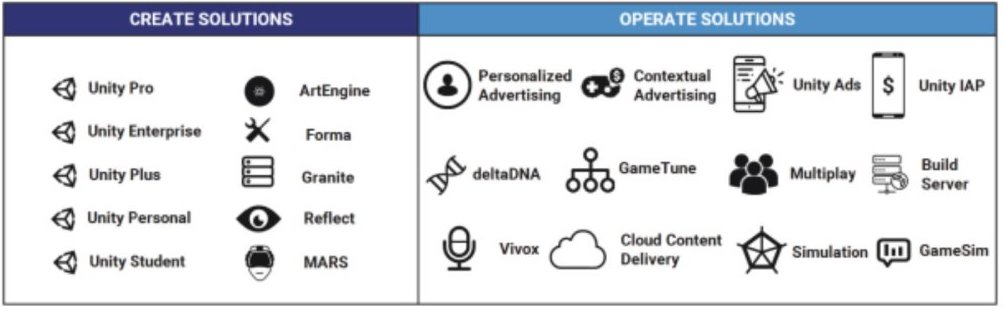
\includegraphics[scale=0.3]{src/thesis/img/background/unity-division.jpg}
    \caption{Products offered in the two organizational divisions of Unity Technologies}
    \label{fig:unity-solutions}
\end{figure}

\begin{itemize}
    \item \textbf{Create solutions}: The main functionality of this product suite is to offer a set of tools that allows users to produce all kinds of 3D content. The business model of this division consists of a subscription-based model for the different versions of the Unity Editor.
    \item \textbf{Operate solutions}: The goal of the products categorized in this section is to enable creators to run a successful business from their 3D content. This is the organizational section that provides the company with the most revenue \cite{UnityRevenue}, and it is also the one that contains UnityAds, the product on which this thesis project was developed.
\end{itemize}

\subsubsection{UnityAds}

UnityAds is one of the most outstanding products offered by the company. To understand it correctly, it is essential to clarify the concept of \textbf{online advertising network} \cite{goldfarb2011online} \cite{schmeiser2016online}. \\

An advertising network is a type of business or service whose purpose is to connect advertisers, who are individuals who want to display advertisements for the products they intend to sell, with publishers, who are individuals who can provide space to place such advertisements, and who usually reach a certain level of audience. The original definition of advertisement network was really tied to newspapers, magazines, and television, but in recent years, it has been extended to online services \cite{ha2008online}. In that sense, UnityAds propose a new innovative business idea because it is an ad-hoc advertisement network for the game industry. In a nutshell, UnityAds allows game developers to show ads about their games in other games and place advertisements of other games in theirs \cite{chu2013iad}. As can be seen, by using UnityAds, the same game developer can be publisher and advertiser simultaneously, melting both roles.\\

\begin{figure}[h]
    \centering
    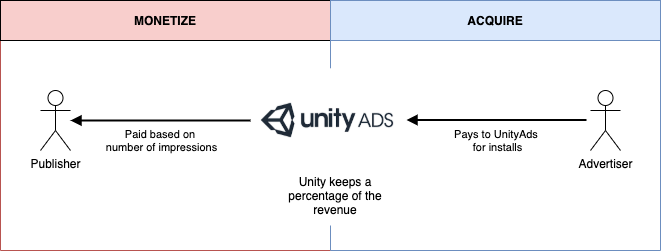
\includegraphics[scale=0.4]{src/thesis/img/background/unity-ads.png}
    \caption{Simplified structure of UnityAds}
    \label{fig:background:unity-ads}
\end{figure}

Figure \ref{fig:background:unity-ads} shows the two aspects that make up the advertising network: \textbf{Acquire} and \textbf{Monetize}. The terms correspond to the classic definition of publisher and advertiser but translated into the gaming industry terminology.

\begin{itemize}
    \item \textbf{Monetize division}: This section includes all the tools provided to game developers to monetize their games, in addition to all the technical solutions needed to deliver an ad to the mobile game that has a publisher space.
    \item \textbf{Acquire division}: This set of tools includes all the products that help advertisers acquire new users who can install the games they advertise on the network.
\end{itemize}

Although this overall context of UnityAds was essential to understand the big picture, only the Acquire division is considered in the following sections, as the thesis project focuses on it.

\subsubsection{Acquire architecture overview}

This section covers the architecture overview for the acquire division of UnityAds. It is important to note that many details of the architecture will not be explained in-depth to respect the company's privacy.\\

The architecture of UnityAds has changed dramatically over the past decade. Initially, the ad network was developed by a Finnish startup, Applifier, acquired by Unity Technologies in 2014 \cite{UnityBuyApplifier}. The initial architecture of the Applifier ad network can be seen in figure \ref{fig:background:applifier-architecture}.

\begin{figure}[h]
    \centering
    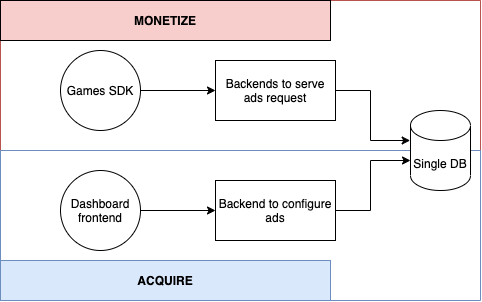
\includegraphics[scale=0.4]{src/thesis/img/background/applifier-unityads-architecture.png}
    \caption{Diagram for the initial architecture of Applifier}
    \label{fig:background:applifier-architecture}
\end{figure}

This almost \textit{monolithic architecture} \cite{de2019monolithic} impacted the startup times, as it was convenient for a small engineering team to introduce changes to it, which allowed them to achieve a solid customer base prior to the Unity acquisition \cite{ApplifierCustomers}. But when scalability started to become a fundamental requirement, there were some pain points they had to address. On the one hand, the database was the junction point between the services and the mechanism they used to communicate, which was limiting and error-prone, and on the other hand, this architecture was not suitable to be managed by a growing team of engineers. Due to this, the company started to migrate its setup into a microservices-oriented architecture (Section CITE-SECTION). This means that now the database is not the single point of communication, and each of the services would need an independent database to store the data they needed to operate. The acquire and monetize division can easily be decoupled using that paradigm, and different teams could work independently. This initiative led the company to its current situation, which can be observed in figure \ref{fig:background:acquire-architecture}.\\

\begin{figure}[h]
    \centering
    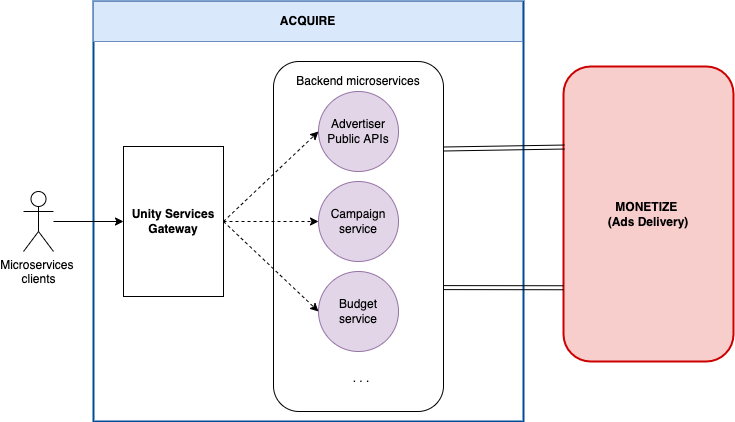
\includegraphics[scale=0.35]{src/thesis/img/background/acquire-division.png}
    \caption{Current architecture of Acquire division of UnityAds}
    \label{fig:background:acquire-architecture}
\end{figure}

On this new setup, Monetization and Acquire can be considered domains on the domain-oriented service architecture of UnityAds (Section CITE-SECTION). It is also important to mention that the communication between microservices uses different protocols; for example, for the public-facing endpoints, the connection is established using HTTPS \cite{durumeric2013analysis}, and for the internal communication between the microservices in the domain, NATS \cite{srisuresh2008state} is the selected protocol, finally, between the monetization and the acquire domains, is Kafka \cite{kreps2011kafka} the chosen technology.\\

One noticeable thing on the diagram is the existence of two gateways as the entry point for the public-facing endpoints. Some of the calls, like the ones provided from the client dashboard, are sent through the legacy gateway, whereas some requests, like those coming from the public APIs, use Unity Services Gateway. The purpose for the existence of two gateways can be traced back some years, while the planning phase of the current domain-oriented service architecture.\\

Before the acquisition of Applifier by Unity, an initial gateway compiled some simple high-level responsibilities (Section CITE-SECTION) that were refactored to add more functionalities like rate limiting, authentication, authorization, and error handling. The legacy gateway is highly tied to the monetization environment, making it difficult to add new functionalities or address pre-existing problems. This is why a new initiative consists of creating a new project, the Unity Services Gateway, whose objective is to serve as the entry point for all the services both on the acquire and monetization domains and possibly across all the company.\\

\subsubsection{Microservices monitoring}

The last step to understand UnityAds architecture is to explain how microservice monitoring is done (Section CITE-SECTION). It is essential to state that all the architecture is deployed on Google Cloud \cite{aceto2013cloud}, which already offers some pre-defined tools that make life easier to operate the product.\\

\begin{figure}[h]
    \centering
    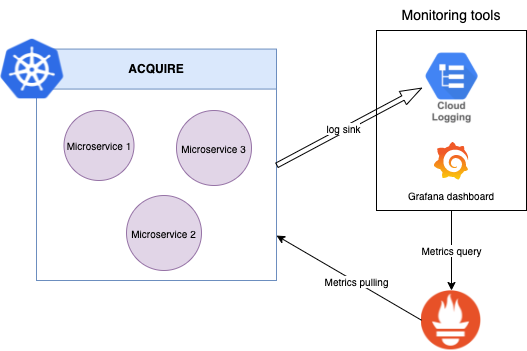
\includegraphics[scale=0.4]{src/thesis/img/background/service-monitoring.png}
    \caption{UnityAds microservices monitoring diagram}
    \label{fig:background:monitoring}
\end{figure}

On figure \ref{fig:background:monitoring} it can be observed a diagram that represents the selected monitoring technologies for the Acquire architecture. As stated before, this architecture is running on a Kubernetes cluster that is deployed on Google Cloud \cite{hunter2018google}. That makes it easier to use log sinks to transfer the logs to the standard google cloud logging tool. But logging is only one of the relevant parts for monitoring, as metrics are also essential to know the overall system's health.\\

In order to collect the metrics for the different microservices of the system, Prometheus \cite{turnbull2018monitoring} is the selected tool. It works by pulling relevant metrics from microservices and infrastructure, and afterward, those metrics can be accessed using its custom query language. On top of it, some Grafana dashboards \cite{hoang2020research} can be handcrafted to visualize those metrics on time series plots. This typical setup works well as it combines the possibility of exploring error logs and even tracing the endpoint calls for the microservices on a fine granularity, using standard Google Cloud tools such as the profiler \cite{thakurratan2018google}, and at the same time presents a visual representation for the metrics of the system, such as error rate, uptime or throughput, using a time-series format.\\

\subsection{Problem definition}

%% Describe the problem from different angles, depending on the stakeholders involved.

%% - Public APIs team: Describe that from our side the requirements is having more
%%                     visibility in the term of the errors that are generating through
%%                     our API calls from the engineering part of view.

%% - Product management: Describe that from the product side, it is important to know the high
%%                       level errors as they are in contact with the client, and they have to 
%%                       contact them in case that they are doing some wrong integrations, for example
%%                       if they hit the rate limits.

%% - Security team: From their perspective it is important to set some visibility on the high level errors
%%                  in case that some individual malicious user is doing some kind of attack to the system.

Even though the monitoring setup adopted by the Acquire unit on UnityAds works well in many cases, it has some limitations related to the monitoring of the Unity Services Gateway. First of all, it is remarkable to say that Unity Services Gateway is another microservice, so the setup represented in figure \ref{fig:background:monitoring} is enough for metrics and architecture monitoring. Nevertheless, it has some limitations for business logic monitoring \cite{von2009decision}.\\

A gateway of a Domain-Oriented microservices architecture is in charge of handling some high-level responsibilities (Section CITE-SECTION). The main advantage is that those tasks are shared across microservices, so there is a single place where this logic is implemented and maintained. But also, the teams responsible for the microservices that are directly dependant on the gateway might want some visibility on the events generated by handling that logic.\\

To give a concrete example for this problem, let's consider only rate-limiting responsibility \cite{raghavan2007cloud}, which is vital to prevent common attacks \cite{jhaveri2012attacks}. The gateway's commitment corresponds to automatically rejecting the requests that had tried to access the server multiple times. To do that, it has to keep a temporal database that stores the count for how many requests the user had done on a concrete time window.\\

Considering this error type, different stakeholders would be interested in knowing more about the events associated with this error and that currently don't have that much information.

\subsubsection*{Public APIs team}

This team is responsible for developing a set of public APIs that allow advertisers to manage their advertisement campaigns programmatically. In Figure \ref{fig:background:acquire-architecture}, it can be seen that the service owned by this team serves as a proxy between the backends and the API client. Usually, those clients are third-party advertisers that have built custom integrations with UnityAds and want to run adverts on different platforms at the same time to maximize the visibility of their campaigns.\\

The engineering team is contacted when some advertiser is constantly receiving errors from the APIs because it has reached the established rate limit for the endpoint they are trying to consume. This can happen for a variety of reasons, maybe they want to fetch a resource that needs multiple calls to be completed, or there is an error in the implementation that causes the endpoint to be called enough times to hit the rate limit. With the current setup, it is tough to trace back the reasons as even if the engineering team can access the logs, as they might not contain all the information in a convenient format. Another drawback is that the engineering team does not notice the problem beforehand, but only after it happens and the clients have already contacted them.

\subsubsection*{Product managers and client partners}

Product managers and client partners are the intermediaries between the engineering team and the clients that consume the APIs or any other connected service through the gateway. This is also why they want to get some visibility in which clients are hitting the rate limits on the gateway level. If they could identify if any client is hitting the rate limits, they can contact them directly to ensure that their integration or their usage of the company's services is correct and give assistance in that regard if needed. In that way, customer satisfaction could be improved with respect to the current status, where is the client who usually contacts if they are experimenting many errors.\\

In that sense, this team is interested in having some visual tool to access that information because accessing the logs console using a series of queries requires some previous background that those professionals might not have.

\subsubsection*{Security team}

The security team wants to know more when specific clients or users make several requests to the services. Because in case that it is not an already identified client, which can be directly contacted, but another malicious user, they can ban him to prevent any further attack \cite{jhaveri2012attacks}.

\clearpage
\section{Requirement analysis}

%% Taking into consideration that everyone has clear who are the stakeholders and what is the structure of the
%% company and the microservices involved, now we have to do the requirement analysis.

%% First of all, it is important to state why it is not possible to store things on Prometheus.

%% We can list the project requirements like:

%% - We need to do a clear definition of the errors that we want to log.
%% - The logging technology has to support a lot of stress as we are having x (collect the number of average requests).
%% - The provided solution has to be cloud agnostic (this is why some part has to be implemented in Terraform or using an external service).
%% - We need a visual tool in order to communicate effectively with the stakeholders.

\subsection{Research questions}

%% Taking into consideration the previous requirement analysis we can state down the research questions.

\clearpage
\section{Literature review}

%% In this section is where all the technologies used are reviewed. For sure having the following subsections:

\subsection{Microservices architectures}

%% In this section we can include the following:
%% - Monolitical vs. microservices architectures. (drawbacks and advantages).
%% - Definition of Domain Oriented Microservices Architecture, stressing out that this is a problem that many 
%%   big companies are facing.

\subsection{Observability \& Monitoring}

%% In this section we can differentiate the following topics:
%% - Observability and Monitoring definition.
%% - Application of observability and monitoring to microservices.
%% - Data observability.
%% - The four pillars of data observability (check one of the articles).

\subsection{Framework comparisons}

%% In this section a comparison of the current frameworks for monitoring and observability has to be done.
%% The following can be compared:

%% - Google custom monitoring & observability tools.
%% - Datadog
%% - Amplitude

%% It is important to explain the features of all of them when monitoring microservices, also taking into consideration
%% the costs analysis, and if they are suitable for showing the custom data that we are going to log.

\clearpage
\section{Technical solution}

%% The outcome of this thesis are basically 4 technical solutions.

\subsection{High level errors definitions}

%% In this section describe the different high level errors and the standard that we are defining for them.
%% Check out the ones defined previously by Uber gateway API.

\subsection{Error schema generator} %%% OPTIONAL

%% Possible Open Source tool used to generate gateway routes schema definitions using a CLI.
%% If implemented, describe it here.

\subsection{Proof of concept using error rate tool}

%% The things that need to be covered here are:

%% - Planning (Using AirTable and estimation)
%% - Implementation on the gateway side. Explain that Unity currently has a logging tool enabled and we only had to log certain events gathering the requests.
%% - Terraform implementation. This part is where it can be explained how we use terraform and how to the problem cloud-agnostic.
%% - BigQuery setup.

\subsection{Error visualization dashboard}

%% Cover here the grafana dashboard implementation tool

%% - Cover the usage of the Grafana + BigQuery tool.
%% - Describe the different panels that had been developed.
%% - Persistance of the dashboard and deployment on every build.

\clearpage
\section{Evaluation}

%% The evaluation needs to be done for each of the artifacts separated:

\subsection{Evaluation of the error schema generator} 

%% Add the testing here if implemented.

\subsection{Evaluation of the proof of concept}

%% Here we can say two evaluation methods:
%% - Test script in order to inject mock data and see if it is storing correctly the data.
%% - Integration tests using jest on the gateway side.
%% - Using Proof of concept in order to test how the database was doing.
%% - Using staging and production in order to have different sources for the data.

\subsection{Evaluation of the visualization tool}

%% For the evaluation of the visualization tool we can explain the following:
%% - Using mock data in order to iterate over the dashboards.
%% - Using continuos reviews from the stakeholders. mention the API team and the gateway team.

\clearpage
\section{Conclusions}

%% This part is almost the last one to write, basically write some pages of conclussions, and offer future work

%% For future work basically it can be checked if there is something on the backlog.

\clearpage
\thesisbibliography

\bibliographystyle{plain}
\bibliography{bibliography}

%% Appendices
%% If you don't have appendices, remove \clearpage and \thesisappendix below.
\clearpage
\thesisappendix

\section{Appendix 1}

\clearpage
\section{Appendix 2}

\clearpage

\end{document}
